\section{Часть II: Сертификаты невыполнимости}

\begin{frame}
    \centering
    \usebeamerfont{title}\insertsectionhead

    \vspace{0.3cm}
    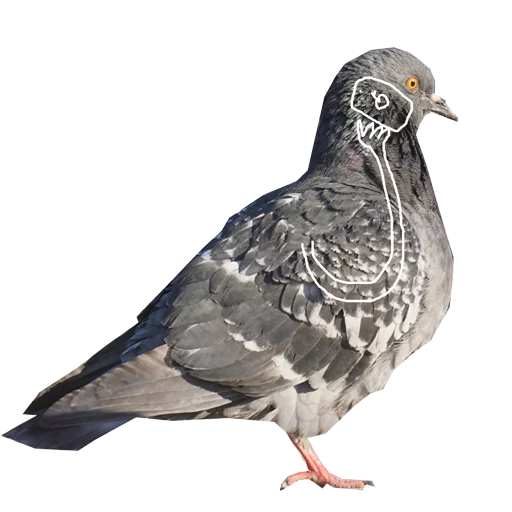
\includegraphics[scale = 0.3]{pics/pigeon1.png}
\end{frame}


\begin{frame}{$\Search_{\varphi}$ [Lov{\'{a}}sz, Naor, Newman, Wigderson et al. 94]}
    
    $\varphi(z) \coloneqq \bigvee\limits_{i = 1}^{m} C_i$~--- невыполнимая формула в КНФ.
    \pause
    
    $\Search_{\varphi} \subseteq \{0, 1\}^n \times [m]$:
    \begin{itemize}
        \item $(\alpha, i) \in \Search_{\varphi} \Leftrightarrow C_{i}(\alpha) = 0.$
    \end{itemize}

    \pause
    \vspace{0.1cm}
    Коммуникационная версия:
    \begin{itemize}
        \item $g\colon X \times Y \to \{0, 1\}$~--- <<гаджет>>;
        \item $\Ind\colon [k] \times \{0, 1\}^k \to \{0, 1\}$, $\Ind(x, y) = y_x$.
    \end{itemize}

    \pause
    \begin{center}
        \begin{tikzpicture}
    \node[thick, circle, draw] (S) at (0, 0) {\Large $S$};
    
    \foreach \i in {1, 2, ..., 5}{
        \node (z\i) at (-3 + \i, -1.5) {$z_{\i}$};
        \draw[->] (z\i) -- (S);
    }
    
    \node[minimum height = 1cm, single arrow, draw] at (3, 0) {composition};

    \node[thick, circle, draw] (S1) at (6, 0) {\Large $S$};

    \foreach \i in {1, 2, ..., 5}{
        \node[draw, circle] (i\i) at (3 + \i, -1.5) {\scriptsize $g$};
        \draw[->] (i\i) -- (S1);

        \node (x\i) at (2.75 + \i, -2.4) {\scriptsize $x_{\i}$};
        \node (y\i) at (3.25 + \i, -2.4) {\scriptsize $y_{\i}$};
        \draw[->] (x\i) -- (i\i);
        \draw[->] (y\i) -- (i\i);
    }
\end{tikzpicture}
    \end{center}


    $\Search_{\varphi} \circ g \equiv \Search_{\varphi \circ g}$.
\end{frame}




\begin{frame}{Системы доказательств}

    \deftext{Резолюция}: доказательство $\varphi \coloneqq \bigvee\limits_{i} C_i$~--- последовательность
    клозов $(D_1, D_2, D_3, \dots, D_{\ell})$:
    \pause
    
    \begin{minipage}{0.3\linewidth}
        \begin{itemize}
            \item $D_i \in \{C_i\}$;
                \pause
            \item $\frac{A \lor x ~~~~~ B \lor \bar{x}}{A \lor B}$, $D_i \coloneqq A \lor B$;
                \pause
            \item $D_{\ell} = \emptyset$.
        \end{itemize}
    \end{minipage}
    \pause
    \begin{minipage}{0.68\linewidth}
        \centering
        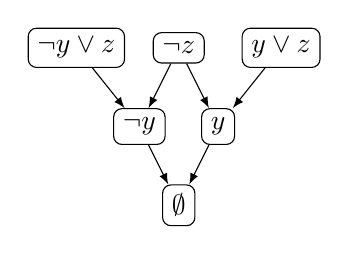
\begin{tikzpicture}[>=latex]
    \node[rectangle, rounded corners = 3pt, draw] (a) at (-1.3, 2)
        {$\neg y \lor z$};
    \node[rectangle, rounded corners = 3pt, draw] (a2) at (1.3, 2)
        {$y \lor z$};
    \node[rectangle, rounded corners = 3pt, draw] (b) at (0, 2)
        {$\neg z$};
    \node[rectangle, rounded corners = 3pt, draw] (c) at (-0.5, 1)
        {$\neg y$};
    \node[rectangle, rounded corners = 3pt, draw] (d) at (0.5, 1)
       {$y$};
    \node[rectangle, rounded corners = 3pt, draw] (e) at (0, 0)
        {$\emptyset$};

    \draw[->] (a) -- (c);
    \draw[->] (a2) -- (d);
    \draw[->] (b) -- (c);
    \draw[->] (b) -- (d);
    \draw[->] (c) -- (e);
    \draw[->] (d) -- (e);
\end{tikzpicture}
    \end{minipage}


    \pause
    \vspace{0.3cm}

    \deftext{Cutting Planes}: доказательство~--- последовательность неравенств над $\mathbb{Z}$
    $(p_1 \ge 0, p_2 \ge 0, p_3 \ge 0, \dots, p_{\ell} \ge 0)$:
    \begin{itemize}
        \item $p_i$ кодировка клоза формулы, $x_k \ge 0$ или $-x_k + 1 \ge 0$;
        \item $\frac{p_i ~~~~~ p_j}{p_k}$, где $p_k$ семантически следует из $p_i$ и $p_j$ на
            $\mathbb{Z}^n$;
        \item $p_{\ell} = 1$.
    \end{itemize}

    \pause
    \vspace{0.3cm}

    \deftext{Nullstellensatz}: доказательство для системы полиномиальных уравнений $f_1 = 0, f_2 = 0,
    \dots$:
    $$
        \sum_{u = 1}^{a} p_u f_u = 1.
    $$
\end{frame}

\begin{frame}{Резолюция и деревья решений}

    \begin{lemma}
        Tree-like резолюция $\Leftrightarrow$ деревья решений для задачи $\Search_{\varphi}$ (не
        коммуникационной).
    \end{lemma}
    \pause

    \begin{minipage}{0.58\linewidth}
        \centering
        \tikzstyle{inner} = [circle, minimum size = 0.3cm, draw, inner sep = 0.1pt]
\tikzstyle{gstyle} = [fill = green]
\tikzstyle{rstyle} = [fill = red]
\tikzstyle{ed} = [->, draw]
\tikzstyle{ops} = [alt=<{#1-}>{opacity = 1}{opacity = 0}]
\tikzstyle{opstyle} = [inner, ops = #1]
\tikzstyle{oped} = [ed, ops = #1]
\tikzstyle{gstyle} = [alt=<{#1}>{fill = green}{}]
\tikzstyle{rstyle} = [alt=<{#1}>{red!90!black}{}]
\tikzstyle{snakestyle} = [
    alt=<{#1}>{
        decorate,
        decoration = {
            snake,
            amplitude = 0.4mm,
            segment length = 2mm,
            post length = 1mm
        }
    }{}]


    
\begin{tikzpicture}[>=latex, xscale = 0.9]
    
    \node[inner, fill = green!30] (a) at (0, 0) {\scriptsize $x$};
    \node[inner, fill = green!30] (b) at (-2, -0.8) {\scriptsize $y$};
    \node[inner] (c) at (2, -0.8) {\scriptsize $a$};
    \node[inner] (d) at (-2.9, -1.6) {};
    \node[inner, fill = green!30] (e) at (-1.1, -1.6) {\scriptsize $z$};
    \node[inner] (f) at (1.1, -1.6) {};
    \node[inner] (g) at (2.9, -1.6) {\scriptsize $w$};

    \node[inner] (h) at (-1.6, -2.4) {};
	\node[inner, fill = green!30] (i) at (-0.6, -2.4) {\scriptsize $u$};
    
    \node[inner] (j) at (2.4, -2.4) {};
    \node[inner] (k) at (3.4, -2.4) {};

    \node[inner, fill = green!30] (l) at (-1, -3.2) {};
    \node[below = 4pt] at (l) {\scriptsize $C_{8}$};
    \node[inner] (m) at (-0.2, -3.2) {};
    
    \draw[ed] (a) -- (b);
    \draw[ed] (a) -- (c);
    \draw[ed] (b) -- (d);
    \draw[ed] (b) -- (e);
    \draw[ed] (c) -- (f);
    \draw[ed] (c) -- (g);
    \draw[ed] (e) -- (h);
    \draw[ed] (e) -- (i);
    \draw[ed] (g) -- (j);
    \draw[ed] (g) -- (k);
    \draw[ed] (i) -- (l);
    \draw[ed] (i) -- (m);
\end{tikzpicture}
    \end{minipage}
    \pause
    \begin{minipage}{0.4\linewidth}
        \centering
        $\frac{A \lor x ~~~ B \lor \neg x}{A \lor B} ~~~~~ \frac{A}{A \lor z}$
        \begin{itemize}
            \item Вершина $\Rightarrow$ дизъюнкция отрицаний запросов.
            \item $(x \lor \neg y \lor \neg z \lor u)$.
        \end{itemize}
    \end{minipage}

    \pause
    $\DCC(\Search_{\varphi \circ g}) \le \DCC(g) \cdot \mathrm{res\text{-}depth}(\varphi).$
\end{frame}


\begin{frame}{Модели}
    \setlength{\extrarowheight}{0.4cm}
        \begin{tabular}{c c c c}
          \textbf{Сис. док.} & \textbf{Модель поиска} & \textbf{Коммуник. модель} & \textbf{Выч. модель}
          \\
          \pause
          Tree Res. & Деревья решений & Комм. протоколы & Мон. формулы \\
          \pause
          Dag-like Res. & Dag решений & Dag протоколы & Мон. схемы \\
          \pause
          CP & ?? & \textcolor{blue}{Dag протоколы} & Вещ. Мон. схемы \\
          \pause
          Tree R(CP) & Stabbing Planes & \textcolor{blue}{Комм. протоколы}  & ?? \\
          \pause
          NS & ?? & Algebraic tiling & Mon. Span Programs \\
        \end{tabular}
    
\end{frame}

\begin{frame}{Лифтинг 
\includegraphics[scale = 0.04]{pics/utia-lift.png}}

    \begin{theorem}[Raz, McKenzie 99; G\"{o}\"{o}s, Pitassi, Watson 16]
        Резолюционная глубина $\varphi$ не менее $d$, тогда:
        $\DCC(\Search_{\varphi} \circ \Ind_m) \ge n^{\bigO{d}},$
        где $m \coloneqq \poly(n)$. \alert{$\DCC(\Search_{\varphi} \circ \Ind_m) \approx
            \DCC(\Ind) \cdot \mathrm{res\text{-}depth}(\varphi)$.}
    \end{theorem}

    Следствие: нижняя оценка на мон. формулы $2^{n^{\varepsilon}}$.
    \pause

    \begin{theorem}[Garg, G\"{o}\"{o}s, Kamath, S 18]
        Резолюционная ширина $\varphi$ не менее $w$, тогда:
        размер dag протокола для $\Search_{\varphi} \circ \Ind_m$ не менее $n^{\bigO{w}},$
        где $m \coloneqq \poly(n)$.
    \end{theorem}

    Следствие: нижняя оценка на мон. \textcolor{blue}{схемы} $2^{n^{\varepsilon}}$.
    \pause

    \begin{theorem}[Pitassi, Robere 16; Robere, Pitassi 18]
        Nullstellensatz степень $\varphi$ не менее $d$, тогда:
        размер \alert{algebraic tiling} для $\Search_{\varphi} \circ g$ не менее $2^{\bigO{w}},$
        для некоторой $g$.
    \end{theorem}

    Следствие: нижняя оценка на мон. Span Programs и мон. формулы $2^{\bigO{n}}$.

\end{frame}